\documentclass[crop,tikz]{standalone}
\usepackage{tikz}
\usetikzlibrary{shapes,arrows,positioning}
\begin{document}
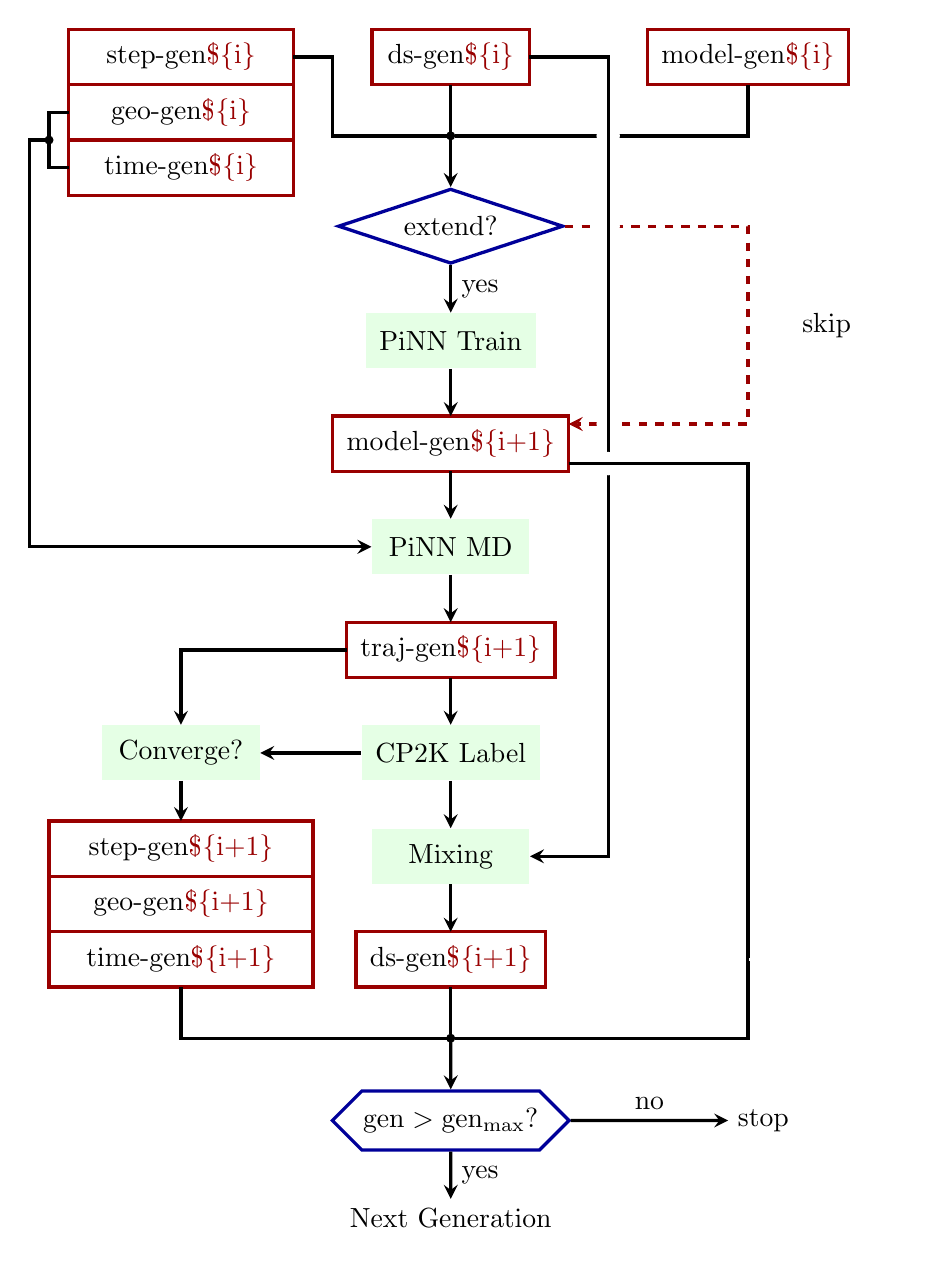
\begin{tikzpicture}[node distance = .6cm, auto]
  \tikzstyle{data} = [rectangle, minimum height=.7cm, minimum width=2cm, draw=red!60!black, very thick, text centered, inner sep=5pt, outer sep=0pt, fill=white]
  \tikzstyle{wf} =   [rectangle, minimum height=.7cm, minimum width=2cm, fill=green!10,  text centered, inner sep=5pt]
  \tikzstyle{line} = [draw,very thick,-stealth]
  \tikzstyle{bdot} = [outer sep=0, inner sep=1, draw, fill, circle]
  \tikzstyle{loop} = [chamfered rectangle, chamfered rectangle xsep=2cm,very thick, draw=blue!60!black, fill=white]
  % Place nodes
  \node [bdot] (train) {};
  \node [data, above=of train] (init-ds) {ds-gen\color{red!60!black}{\$\{i\}}};
  \node [data, text width=2.5cm, left=1cm of init-ds] (init-step) {step-gen\color{red!60!black}{\$\{i\}}};
  \node [data, text width=2.5cm, below=0 of init-step] (init-geo) {geo-gen\color{red!60!black}{\$\{i\}}};
  \node [data, text width=2.5cm, below=0 of init-geo] (init-time) {time-gen\color{red!60!black}{\$\{i\}}};
  \node [diamond, below=of train, draw=blue!60!black, very thick, aspect=3] (iftrain) {extend?};
  \node [data, right=1.5cm of init-ds] (init-model) {model-gen\color{red!60!black}{\$\{i\}}};
  \node [wf, below=of iftrain] (train2) {PiNN Train};
  \node [data, below=of train2, text width=] (model) {model-gen\color{red!60!black}{\$\{i+1\}}};
  \node [wf, below=of model] (emd) {PiNN MD};
  \node [data, below=of emd, text width=] (traj) {traj-gen\color{red!60!black}{\$\{i+1\}}};
  \node [wf, below=of traj] (cp2k) {CP2K Label};
  \node [wf, below=of cp2k] (mix) {Mixing};
  \node [wf] (conv) at (cp2k -| init-geo) {Converge?};
  \node [data, below=of mix, text width=] (new-ds) {ds-gen\color{red!60!black}{\$\{i+1\}}};
  \node [data, text width=3cm,] (new-time) at (new-ds -| conv)  {time-gen\color{red!60!black}{\$\{i+1\}}};
  \node [data, text width=3cm, above=0 of new-time] (new-geo) {geo-gen\color{red!60!black}{\$\{i+1\}}};
  \node [data, text width=3cm, above=0 of new-geo] (new-step) {step-gen\color{red!60!black}{\$\{i+1\}}};
  %\node [data, text width=] (new-model) at (new-ds -| init-model)  {model-gen{\color{red!60!black}\$\{i+1\}}};
  %\node [data, dashed] at (iftrain-|new-model) (copy-model) {\color{white}model-gen{\$\{i\}}};
  \node [inner sep=0, outer sep=0,fill] (new-model) at (new-ds -| init-model)  {};

  \path [line,-] (init-ds) -- (train);
  \path [line,-] (init-model) |- (train);
  \path [line] (train) -- (iftrain);
  \path [line] (iftrain) -- (train2) node [midway] {yes};
  \path [line] (train2) -- (model);
  \path [line] (model) -- (emd);
  \path [line] (emd) -- (traj);
  \path [line] (traj) -- (cp2k);
  \path [data, dashed, -stealth] (iftrain) -- (iftrain-|init-model) -- ([yshift=-0.1cm]init-model|-model.north)
  node [midway] {skip} -- ([yshift=-0.1cm]model.north east);
  \node [outer sep=0, inner sep=3, fill=white, circle] at ([xshift=1cm,yshift=-0.1cm]init-ds.east|-model.north) {};
  \node [outer sep=0, inner sep=3, fill=white, circle] at ([xshift=1cm]init-ds.east|-train) {};
  \node [outer sep=0, inner sep=3, fill=white, circle] at ([xshift=1cm]init-ds.east|-iftrain) {};
  \path [line] (init-ds) -| ([xshift=1cm]init-ds.east) |-(mix);
  \node [bdot] at ([xshift=-.25cm]init-geo.south west) {};
  \node [outer sep=0, inner sep=3, fill=white, circle] at ([xshift=1cm,yshift=0.1cm]init-ds.east|-model.south) {};
  \path [line,-] (init-step) -- ([xshift=.5cm]init-step.east) |-(train);
  \path [draw, very thick] (init-geo) -- ([xshift=-.25cm]init-geo.west) -- ([xshift=-.25cm]init-geo.south west);
  \path [draw, very thick] (init-time) -- ([xshift=-.25cm]init-time.west) -- ([xshift=-.25cm]init-time.north west);
  \path [line] ([xshift=-.25cm]init-time.north west) -- ([xshift=-.5cm]init-time.north west) |- (emd);
  \path [line] (cp2k) -- (mix);
  \path [line] (traj) -| (conv);
  \path [line] (cp2k) -- (conv);
  \path [line] (mix) -- (new-ds);
  \path [line] (conv) -- (new-step);
  % \path [data, -, dashed] (copy-model) -- (model.north east);

  \path [line,-] ([yshift=0.1cm]model.south east) -| (new-model);
  \node [below=of new-ds, bdot] (new-all) {};
  \node[below=of new-all, loop, align=center] (ifnext){$\mathrm{gen}>\mathrm{gen_{max}}$?};
  \path [line,-] (new-ds) -- (new-all);
  \path [line,-] (new-time) |- (new-all);
  \path [line,-] (new-model) |- (new-all);
  \path [line] (new-all) -- (ifnext);
  \node[below=of ifnext] (next) {Next Generation};
  \path [line] (ifnext) -- (next) node [midway] {yes};
  \node[right= 2cm of ifnext] (stop) {stop};
  \path [line] (ifnext) -- (stop) node [midway] {no};
\end{tikzpicture}
\end{document}
